% ============================================================
%  VialServi - Documento de sustentacion
%  Proyecto Integrador 2026-2
%  Compilar: pdflatex Sustentacion-VialServi.tex  (dos veces)
% ============================================================
\documentclass[12pt,letterpaper]{article}

\usepackage[utf8]{inputenc}
\usepackage[T1]{fontenc}
\usepackage[spanish,es-nodecimaldot]{babel}
\usepackage{mathptmx}
\usepackage{graphicx}
\usepackage{float}
\usepackage{setspace}
\usepackage{tabularx}
\usepackage{array}
\usepackage{enumitem}
\usepackage{fancyhdr}
\usepackage{xcolor}
\usepackage{tcolorbox}
\usepackage[hyphens]{url}
\usepackage[hidelinks]{hyperref}
\Urlmuskip=0mu plus 1mu

\usepackage[top=3.5cm, bottom=2cm, left=3cm, right=1.9cm,
            headheight=2.6cm, headsep=0.6cm, footskip=1cm]{geometry}

\setlength{\parindent}{1.27cm}
\setlength{\parskip}{0pt}
\onehalfspacing

\definecolor{ambar}{HTML}{B45309}
\definecolor{grisclaro}{HTML}{F4F4F5}

% ── Datos del formato ───────────────────────────────────────
\newcommand{\formatoTitulo}{\shortstack{PROYECTO INTEGRADOR\\
  VialServi · Documento de sustentación}}
\newcommand{\formatoCodigo}{PI--2026--2}
\newcommand{\formatoVersion}{01}

\pagestyle{fancy}
\fancyhf{}
\renewcommand{\headrulewidth}{0pt}
\fancyhead[C]{%
  \setlength{\tabcolsep}{4pt}%
  \renewcommand{\arraystretch}{1.2}%
  \begin{tabularx}{\textwidth}{|>{\centering\arraybackslash}m{3.9cm}
                               |>{\centering\arraybackslash}X
                               |>{\centering\arraybackslash}m{3.1cm}|}
    \hline
    
\includegraphics[width=3.4cm]{logo-poli.jpeg} &
    \small\textbf{\formatoTitulo} &
    {\footnotesize\shortstack{Código: \formatoCodigo\\ Versión: \formatoVersion}} \\
    \hline
  \end{tabularx}}
\fancyfoot[C]{\small\thepage}

% ── Hoja horizontal para el mapa ────────────────────────────
\newcommand{\paginaancha}{%
  \clearpage
  \pdfpagewidth=11in \pdfpageheight=8.5in
  \newgeometry{top=3.5cm, bottom=2cm, left=2.5cm, right=2.5cm,
               headheight=2.6cm, headsep=0.6cm, footskip=1cm}}
\newcommand{\paginanormal}{%
  \clearpage
  \pdfpagewidth=8.5in \pdfpageheight=11in
  \restoregeometry}

% ── Estilos de titulo: cada seccion empieza en pagina nueva ─
\makeatletter
\renewcommand{\section}[1]{%
  \clearpage
  \refstepcounter{section}%
  \vspace*{0.2\baselineskip}%
  {\raggedright\Large\bfseries\thesection.\; #1\par}%
  \addcontentsline{toc}{section}{\thesection.\; #1}%
  \vspace{0.8\baselineskip}}
\renewcommand{\subsection}[1]{%
  \refstepcounter{subsection}%
  \vspace{0.9\baselineskip}%
  {\raggedright\large\bfseries\thesubsection\; #1\par}%
  \addcontentsline{toc}{subsection}{\thesubsection\; #1}%
  \vspace{0.3\baselineskip}}
\makeatother

\newtcolorbox{clave}[1][]{colback=grisclaro, colframe=ambar, boxrule=0.8pt,
  arc=2pt, left=8pt, right=8pt, top=6pt, bottom=6pt, #1}

\setlist[itemize]{leftmargin=1.1cm, itemsep=2pt, topsep=4pt, parsep=0pt}
\setlist[enumerate]{leftmargin=1.1cm, itemsep=2pt, topsep=4pt, parsep=0pt}

\newcommand{\tablita}[1]{\begin{center}\small\singlespacing #1\end{center}}

\begin{document}

% ── Portada ─────────────────────────────────────────────────
\thispagestyle{fancy}
\begin{center}
  \vspace*{2.5cm}
  {\LARGE\bfseries VialServi\par}
  \vspace{0.5cm}
  {\large\bfseries Aplicativo web para la gestión de expedientes de servicios\\
  mecánicos, de cerrajería, de grúa y de conductor elegido\par}

  \vspace{1cm}
  {\large Documento de sustentación\par}

  \vspace{2.5cm}
  Edwin Andrés Sánchez Orozco\\
  Brahian Estiven Rendón Murillo\\
  Juan Pablo Vásquez Marín

  \vspace{1cm}
  Facultad de Ingenierías\\
  Politécnico Colombiano Jaime Isaza Cadavid

  \vspace{1cm}
  Proyecto Integrador\\
  Claudia Alejandra Rosero Noguera

  \vspace{1cm}
  \today
\end{center}
\clearpage

% ── Indice ──────────────────────────────────────────────────
\thispagestyle{fancy}
{\Large\bfseries Contenido\par}
\vspace{0.6cm}
{\singlespacing
\makeatletter
\@starttoc{toc}
\makeatother
}

\section{El problema y la solución}

VialServi presta servicios de asistencia mecánica, cerrajería, traslado en grúa y
conductor elegido. Cada atención genera información que después resulta
indispensable: quién atendió, en qué estado se recibió el vehículo, qué objetos
había dentro, cuánto duró la atención y qué novedades se presentaron.

Hoy esa información se recoge a mano y queda dispersa: cuadernos que lleva cada
técnico, fotografías en celulares personales y mensajes de WhatsApp a la central.
No existe un lugar único donde consultar el historial de un servicio.

\begin{clave}
\textbf{La consecuencia concreta.} Cuando un cliente reclama un objeto de valor o
una aseguradora pide el soporte de un servicio prestado semanas atrás, la empresa
no siempre tiene con qué responder, porque las fotografías quedaron en el celular
de un técnico que las borró o cambió de equipo. La empresa estima esa pérdida en
cerca de \$3.200.000 mensuales entre servicios no facturables y reclamaciones sin
evidencia.
\end{clave}

La solución es un aplicativo web donde cada servicio queda registrado en un
\textbf{expediente único}, alojado en línea, disponible para la empresa en
cualquier momento y sin depender del dispositivo personal de nadie.

\subsection{Alineación con el desarrollo sostenible}

El proyecto se alinea con el Objetivo de Desarrollo Sostenible número 9, Industria,
Innovación e Infraestructura, al llevar transformación digital a un sector que
trabaja de forma manual. De manera complementaria aporta al Objetivo 12,
Producción y Consumo Responsables, al reemplazar formularios físicos por registros
digitales.

\subsection{Por qué se dice ``servicios mecánicos, de cerrajería, de grúa y de
conductor elegido'' y no ``asistencia vial''}

Es una precisión deliberada. ``Asistencia vial'' es un término que abarca desde un
cambio de llanta hasta la atención de un siniestro con heridos. VialServi
\textbf{no presta atención médica de emergencia} ni interviene en accidentes con
lesionados. Nombrar los cuatro servicios concretos delimita el alcance y evita que
se le atribuyan al proyecto responsabilidades que no tiene.

\section{Alcance del proyecto}

El alcance se organiza por módulos siguiendo el orden lógico en que ocurre un
servicio: primero el vehículo, que es el punto de partida porque sin vehículo no
hay servicio; luego el cliente al que pertenece; después el servicio que ese
cliente solicita y que la central clasifica; y por último el expediente, que
concentra toda la información de la atención.

\subsection{Los módulos}

\tablita{
\begin{tabularx}{\textwidth}{|>{\raggedright\arraybackslash}p{4.3cm}|>{\raggedright\arraybackslash}X|}
\hline
\textbf{Módulo} & \textbf{Qué hace} \\ \hline
Seguridad y control de acceso &
Inicio de sesión, registro, recuperación y cambio de contraseña, y
administración de usuarios, roles y permisos. \\ \hline
Gestionar vehículo e inventario &
Placa, marca, modelo, color y propietario, junto con el inventario de los objetos
que quedan dentro del vehículo. Es el punto de partida del sistema: el cliente
registra el suyo y la central registra el de cualquiera. \\ \hline
Gestionar cliente &
Datos del cliente al que pertenece el vehículo. El expediente enlaza esta
información; no la duplica. \\ \hline
Gestionar técnico &
El técnico se administra como entidad propia y no solo como rol de usuario, porque
su hoja de vida —especialidades, certificaciones y licencia— determina qué
servicios puede atender. \\ \hline
Gestionar servicio &
Solicitud del cliente y clasificación por parte de la central en los tres tipos:
traslado en grúa (vehículo y pasajeros), carro taller (mecánica en sitio, cambio
de llantas y cerrajería) y conductor elegido, disponible 24 horas. \\ \hline
Gestionar expediente &
Módulo central. Se abre al clasificar el servicio y concentra la información del
vehículo, el cliente, el servicio y el técnico. Sobre él se diligencia el formato,
se cargan evidencias, se registra el inventario y se reportan novedades. \\ \hline
Gestionar históricos y reportes &
Almacenamiento de los expedientes cerrados, consulta del historial por placa y
panel de indicadores de la operación. \\ \hline
\end{tabularx}}

\subsection{Retención y archivado}

Cada expediente cerrado permanece disponible de forma activa mientras la empresa
lo requiera para reclamaciones o auditorías. Como este tipo de soportes suele
exigirse por varios años, \textbf{el sistema no elimina información por sí solo}:
los expedientes vencidos se archivan, no se borran, y la decisión de depurarlos
queda en manos de la empresa.

\subsection{Lo que este proyecto no incluye}

\begin{itemize}
  \item Contratación de personal, compra de equipos móviles o mejoras en la
        cobertura celular: son decisiones de la organización, no del software.
  \item Atención de accidentes de tránsito con heridos o intervención de entidades
        de salud y de tránsito. VialServi presta asistencia mecánica, técnica y de
        grúa, no atención médica de emergencia.
\end{itemize}

\subsection{Dependencia entre módulos}

El expediente no puede existir por sí solo: para abrirlo se necesita primero el
vehículo y el cliente enlazado a él, y para cerrarlo se necesita el registro del
técnico que lo atendió. Por eso el orden de construcción de los módulos sigue el
mismo orden del flujo del servicio y no al contrario.

\section{Objetivos}

\subsection{Objetivo general}

Construir un aplicativo web para la gestión de los servicios de carro taller (mecánica y cerrajería), traslado
en grúa de vehículos y pasajeros, y conductor elegido que presta VialServi, en el
que cada servicio quede registrado en un expediente único, con el formato que le
corresponde y con acceso controlado por roles, desde que el cliente lo solicita
hasta que la central lo cierra, con el fin de que la evidencia de cada atención
esté siempre disponible para la empresa y no dependa de los dispositivos
personales de los técnicos.

\subsection{Objetivos específicos}

Siguen las fases clásicas del ciclo de vida del desarrollo de software: análisis,
diseño, construcción y pruebas.

\begin{itemize}
  \item Analizar las necesidades de información de la empresa y los requisitos que
        debe cumplir el sistema, tanto en sus funciones principales como en
        aspectos de seguridad y desempeño.
  \item Diseñar la arquitectura de la plataforma y el modelo de la base de datos,
        dejando documentadas las decisiones tomadas y las razones detrás de cada
        una.
  \item Construir los módulos funcionales del sistema, incluyendo el registro de
        expedientes, la carga de evidencias, el inventario de objetos de valor y
        el control de acceso por roles.
  \item Verificar el correcto funcionamiento del sistema construido, mediante
        pruebas que confirmen su fiabilidad, seguridad y usabilidad conforme a los
        criterios de calidad de software reconocidos internacionalmente.
\end{itemize}

\section{Mapa de navegación}

El mapa representa los módulos del aplicativo y el orden en que fluye la
información entre ellos. Concentra la información en un solo nivel de módulos: los
roles no se ramifican, porque la asignación de permisos se resuelve en el back-end
y no en la navegación. Las flechas numeradas siguen el recorrido de un servicio,
desde el vehículo hasta los reportes.

\paginaancha
\begin{figure}[H]\centering
  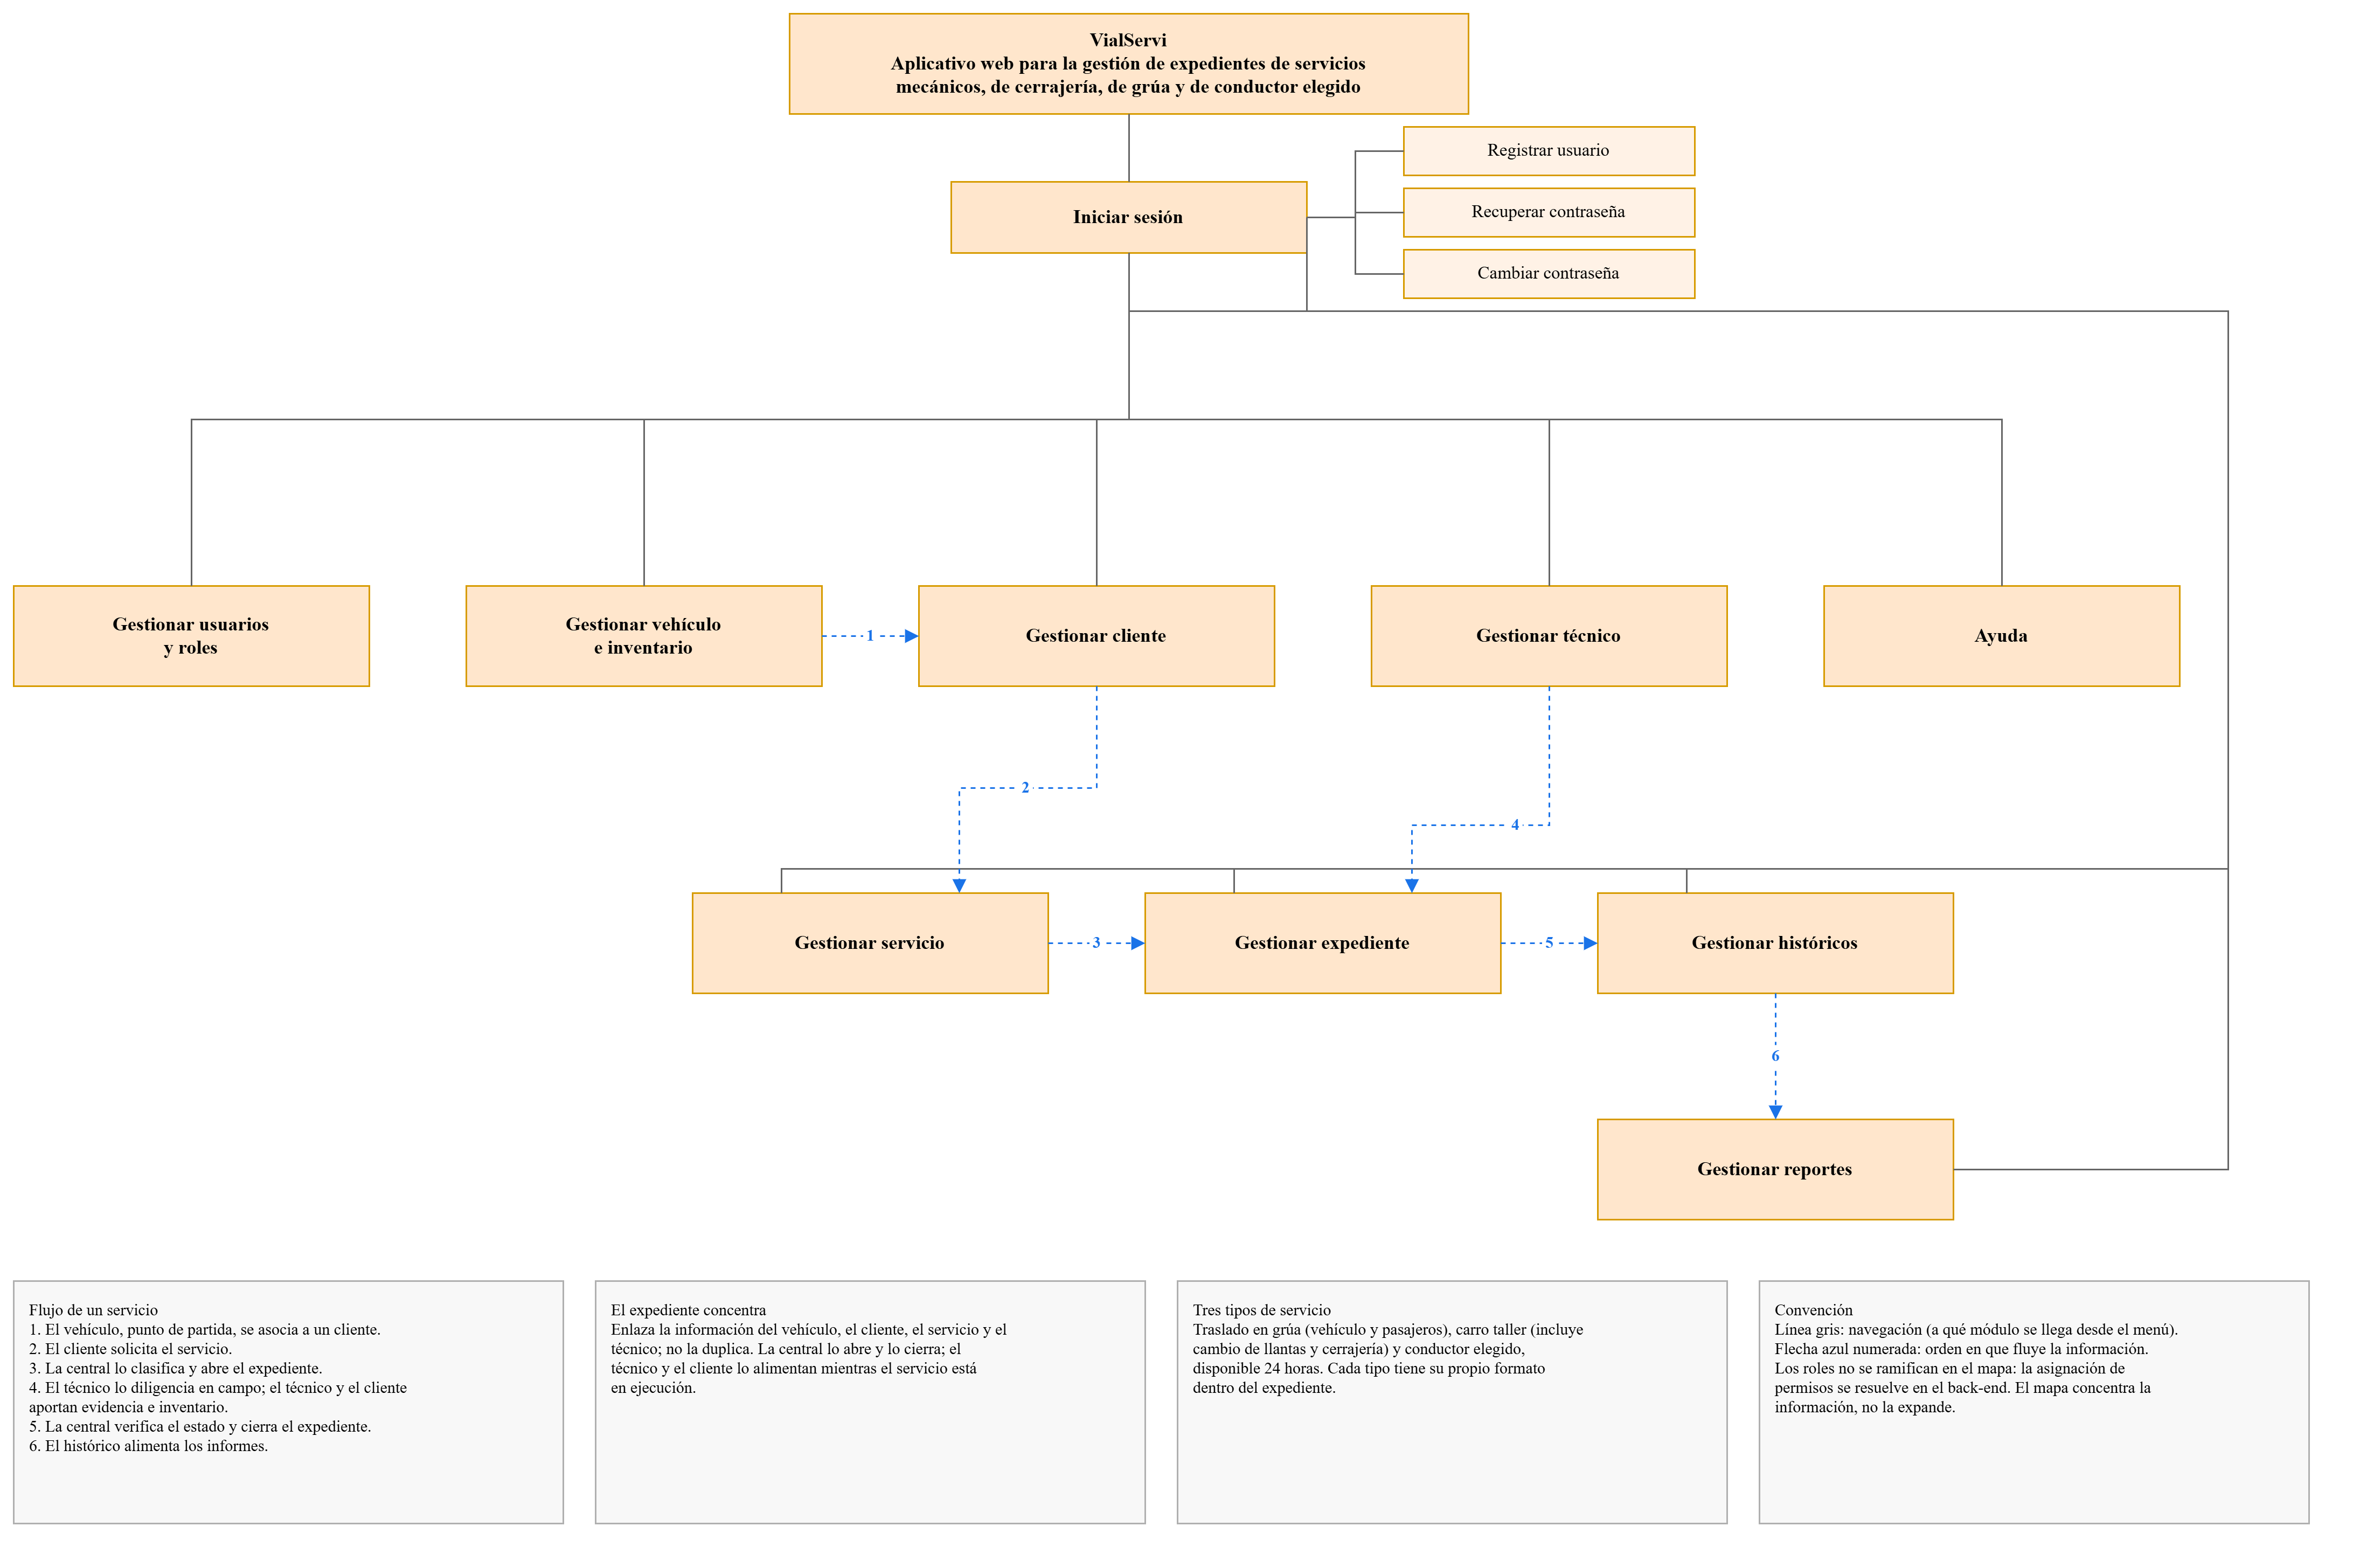
\includegraphics[width=22cm]{mapa.png}
  \caption{Mapa de navegación del aplicativo VialServi.}
\end{figure}
\paginanormal

\section{Correcciones aplicadas tras la asesoría}

Esta sección deja explícito qué se observó, qué se cambió y dónde se puede
verificar. Es la parte que conviene tener presente en la sustentación.

\tablita{
\begin{tabularx}{\textwidth}{|>{\raggedright\arraybackslash}p{4.6cm}|>{\raggedright\arraybackslash}X|}
\hline
\textbf{Observación recibida} & \textbf{Qué se cambió} \\ \hline
El mapa ramificaba los roles; con muchos usuarios sería imposible de dibujar, y
los permisos son asunto del back-end, no de la navegación &
Los roles quedaron concentrados en un solo módulo. El mapa ya no los expande, y la
convención del diagrama lo declara por escrito \\ \hline
El orden de los módulos no reflejaba el proceso real del negocio &
El mapa sigue ahora el orden lógico: vehículo $\rightarrow$ cliente $\rightarrow$
servicio $\rightarrow$ expediente $\rightarrow$ históricos $\rightarrow$ reportes,
con las relaciones numeradas de 1 a 6 \\ \hline
El punto de partida de todo es el vehículo: sin vehículo no hay servicio &
``Gestionar vehículo e inventario'' es el primer módulo del flujo, y el alcance lo
declara explícitamente \\ \hline
El técnico no es solo un rol: tiene hoja de vida con especialidades que determinan
qué puede atender &
``Gestionar técnico'' es un módulo y una entidad propia, con especialidades y
licencia. Al asignar, el sistema solo ofrece técnicos aptos y disponibles \\ \hline
Faltaba decir cuándo y quién cierra un servicio &
Los estados quedaron definidos, y el cierre es exclusivo de la central, con
condiciones verificables \\ \hline
``Interfaz para el técnico de campo'' era una lista de requisitos no funcionales,
no de funcionalidades &
Ese falso módulo se eliminó del alcance. La usabilidad en celular se trata como
requisito no funcional \\ \hline
Unificar la terminología &
Lo que se llamaba ``gestión de evidencias y novedades'' se llama
\textbf{expediente} en todo el documento, el código y el diagrama \\ \hline
``Asistencia vial'' es ambiguo: sugiere atención de siniestros con heridos &
Se nombran los servicios concretos en el título, el objetivo general y el mapa, y
se añadió la exclusión explícita de accidentes con heridos \\ \hline
No es una página web, es un aplicativo web &
Corregido en todo el documento, el título y el diagrama \\ \hline
El trabajo sin señal hay que implementarlo, no excluirlo &
Salió de las exclusiones y entró al alcance, con un diseño acotado y realizable
que se explica en la sección 7 \\ \hline
\end{tabularx}}

\section{Arquitectura}

Un aplicativo web son en realidad dos programas separados que se comunican.

\begin{verbatim}
   NAVEGADOR DEL USUARIO                    SERVIDOR

   +------------------+   petición    +----------------+   +----------+
   |   Frontend       | ------------> |   Backend      |-->|  Base    |
   |   lo que se ve   |               |  lo que decide |   | de datos |
   |                  | <------------ |   y valida     |<--|          |
   +------------------+   respuesta   +----------------+   +----------+
\end{verbatim}

El \textbf{frontend} es lo que el usuario ve y toca. El \textbf{backend} es lo que
decide y guarda. El punto de contacto se llama \textbf{API}: la ventanilla por la
que el frontend pide y el backend responde.

\begin{clave}
\textbf{Por qué importa esta separación.} Las reglas del negocio viven en el
backend, donde el usuario no las puede tocar. Si ocultáramos un botón en la
pantalla pero la regla no estuviera en el servidor, cualquiera con conocimientos
básicos podría saltársela. En la sección 9 se muestra que esto no es una
afirmación: está probado.
\end{clave}

\section{El expediente: ciclo de vida y reglas}

\subsection{Quién escribe qué}

\tablita{
\begin{tabularx}{\textwidth}{|>{\raggedright\arraybackslash}X|>{\raggedright\arraybackslash}p{4.6cm}|}
\hline
\textbf{Dato} & \textbf{Quién lo escribe} \\ \hline
Solicitud: dirección, descripción, vehículo & Cliente, o Central si llamó por teléfono \\ \hline
Tipo de servicio y técnico asignado & Central \\ \hline
Consecutivo y apertura del expediente & El sistema, al clasificar \\ \hline
Observaciones del expediente & Técnico \\ \hline
Evidencias (fotografía o video de máximo 10 segundos) & Técnico \textbf{y} Cliente \\ \hline
Novedades e inventario del vehículo & Técnico \\ \hline
Cierre: fecha y responsable & \textbf{Solo Central} \\ \hline
Cancelación con motivo & Central \\ \hline
Usuarios, roles y hoja de vida del técnico & Administrador \\ \hline
\end{tabularx}}

\begin{clave}
\textbf{El técnico y la central no comparten ni un solo campo del expediente.} Esa
es la razón por la que una actualización del técnico nunca puede sobrescribir el
cierre hecho por la central. No hay conflicto porque no hay terreno compartido.
\end{clave}

\subsection{Estados del servicio}

\begin{verbatim}
 SOLICITADO --> ASIGNADO --> EN_EJECUCION --> TERMINADO --> CERRADO
      |             |              |
      +-------------+--------------+------------------> CANCELADO
\end{verbatim}

El técnico avanza de \emph{asignado} a \emph{en ejecución} y de ahí a
\emph{terminado}, porque son hechos que solo él conoce en el sitio. Solo la central
pasa a \emph{cerrado}: quien presta el servicio no declara cerrada la evidencia de
que existió. Eso se llama \textbf{separación de funciones}.

La cancelación exige motivo, porque un servicio que desaparece sin explicación es
justamente el hueco de trazabilidad que el sistema busca evitar. Un servicio ya
cerrado no se puede cancelar.

\subsection{Un recorrido completo}

\begin{enumerate}
  \item El cliente solicita el servicio indicando dirección, descripción y
        vehículo.
  \item La central lo clasifica en uno de los tres tipos y lo asigna a un técnico
        apto. En ese momento nace el expediente con su consecutivo.
  \item El técnico marca \emph{en ejecución} al llegar al sitio.
  \item Diligencia el formato del tipo de servicio, registra el inventario del
        vehículo, carga las evidencias y anota las novedades. El cliente puede
        aportar sus propias fotografías.
  \item El técnico marca \emph{terminado}.
  \item La central verifica y cierra el expediente.
  \item El expediente cerrado alimenta el histórico y los indicadores.
\end{enumerate}

\subsection{La evidencia del cliente}

El cliente puede aportar sus propias fotografías al expediente de su servicio, y
cada evidencia guarda \textbf{quién la subió}. Ante una reclamación por un rayón,
el expediente muestra las dos versiones con su autor y su hora: las del cliente
antes del traslado y las del técnico durante la atención. Sin ese dato, las
fotografías serían indistinguibles y el expediente no resolvería la disputa.

\subsection{Evidencia que llega después del cierre}

Si una evidencia llega cuando la central ya cerró, \textbf{no se rechaza}: se
guarda marcada como posterior al cierre. El criterio es que perder evidencia es
peor que tener un registro tardío, y en una reclamación esa fotografía puede ser
justamente la que importa.

\section{El trabajo sin señal}

El técnico atiende en carretera, donde la cobertura falla. El aplicativo debe
permitirle registrar sin conexión y enviar después.

\subsection{El error que hay que evitar}

La forma intuitiva es construir dos modos: uno conectado que guarda en el servidor
y otro desconectado que guarda en el celular. Eso obliga a escribir la misma
lógica dos veces y, al reconectar, a comparar dos versiones de la verdad y decidir
cuál gana. Ahí es donde este tipo de solución se vuelve inabordable.

\subsection{El diseño: un solo camino}

\begin{verbatim}
        El técnico pulsa "Guardar"
                   |
                   v
        +---------------------+
        |  BUZÓN DE SALIDA    |  Siempre se escribe aquí primero,
        |  (IndexedDB)        |  haya señal o no. Sin excepción.
        +----------+----------+
                   |
             ¿hay conexión?
              |          |
             SÍ          NO
              |          |
              v          v
        se envía     queda pendiente
        al API       ("2 sin enviar")
              |          |
              |          +--> al volver la señal
              |               se reintenta solo
              v
        el servidor confirma  -->  se borra del buzón
\end{verbatim}

Con señal ese recorrido dura milisegundos y el técnico no nota que el buzón
existe. Sin señal, el registro espera. \textbf{Es el mismo código en ambos casos.}

\subsection{Por qué no hay conflictos}

\begin{enumerate}
  \item \textbf{Casi todo lo que hace el técnico son inserciones, no ediciones.}
        Una fotografía, una novedad, un objeto del inventario: cada uno es una fila
        nueva. Dos filas nuevas jamás se pisan.
  \item \textbf{Los campos están repartidos por rol}, como se mostró en la sección
        anterior.
  \item \textbf{La sincronización va en un solo sentido}, del dispositivo al
        servidor. No se bajan cambios para fusionarlos, de modo que la pregunta
        ``¿cuál versión gana?'' no llega a plantearse.
\end{enumerate}

\subsection{Reintentar no es lo mismo que un conflicto}

Cada registro viaja con un identificador generado en el dispositivo. Si la
petición se reintenta diez veces, el servidor reconoce que ya tiene ese registro y
no lo duplica. Para el único campo que el técnico edita —las observaciones— existe
además un contador de versión: el servidor descarta cualquier actualización cuyo
contador sea menor al guardado, de modo que un envío viejo que llega tarde no pisa
el texto nuevo.

Se usa un contador y no la hora del dispositivo porque un reloj mal configurado
podría revertir una edición más reciente.

\subsection{Casos analizados}

\tablita{
\begin{tabularx}{\textwidth}{|>{\raggedright\arraybackslash}p{5.2cm}|>{\raggedright\arraybackslash}X|}
\hline
\textbf{Caso} & \textbf{Comportamiento} \\ \hline
Registro reintentado muchas veces & El identificador del dispositivo hace que se aplique una sola vez \\ \hline
Expediente creado sin señal y evidencias de ese expediente & Las evidencias referencian al padre por su identificador local; la cola envía el padre primero \\ \hline
Evidencia que llega tras el cierre & Se acepta y se marca \\ \hline
Registro inválido que el servidor rechaza siempre & Tras varios intentos se aparta como ``requiere revisión''; la cola no se bloquea \\ \hline
Se cierra el navegador o se agota la batería & El buzón vive en la base del navegador, no en memoria: al reabrir sigue ahí \\ \hline
Dos pestañas sincronizando a la vez & El identificador único descarta el duplicado \\ \hline
Reloj del dispositivo mal configurado & Para las observaciones manda el contador, no la hora \\ \hline
Orden de llegada de las evidencias & Se muestran por la hora en que se tomaron, no por la de llegada \\ \hline
\end{tabularx}}

\subsection{Qué cubre y qué no}

Cubre el registro en campo: diligenciar el formato, tomar fotografías, grabar
clips de máximo diez segundos y anotar novedades sin cobertura. \textbf{No cubre}
la consulta del histórico completo sin conexión, que sí requiere red.

\section{Tecnologías}

Todas tienen licencia libre o un plan gratuito suficiente para el proyecto, de modo
que su implantación no depende de un presupuesto.

\tablita{
\begin{tabularx}{\textwidth}{|>{\raggedright\arraybackslash}p{2.6cm}|>{\raggedright\arraybackslash}p{4.2cm}|>{\raggedright\arraybackslash}X|}
\hline
\textbf{Capa} & \textbf{Tecnología} & \textbf{Para qué se usa} \\ \hline
Lenguaje & TypeScript & Único lenguaje del proyecto, en servidor e interfaz \\ \hline
Servidor & Node.js con Express & API por la que se exponen los módulos \\ \hline
Validación & Zod & Revisa los datos antes de que lleguen a la base \\ \hline
Base de datos & Prisma ORM sobre SQLite, portable a PostgreSQL & Esquema, migraciones versionadas y consultas \\ \hline
Seguridad & JWT y bcrypt & Sesiones con vencimiento y contraseñas cifradas \\ \hline
Interfaz & React con Vite & Pantallas del aplicativo \\ \hline
Estilos & Tailwind CSS & Diseño, incluida la vista del técnico en celular \\ \hline
Estado y datos & TanStack Query & Consulta al API con caché y manejo de errores \\ \hline
Pruebas & Vitest y Supertest & Pruebas automatizadas del API \\ \hline
Pruebas manuales & Postman & Prueba de cada ruta durante el desarrollo \\ \hline
Nube & Supabase & PostgreSQL gestionado y almacenamiento de fotografías \\ \hline
Sin señal & Dexie.js sobre IndexedDB & Buzón de salida en el dispositivo \\ \hline
Instalable & vite-plugin-pwa & Permite que el aplicativo abra sin señal \\ \hline
Versiones & Git & Historial del código y la documentación \\ \hline
Ejecución & Node.js 20 y npm workspaces & Servidor e interfaz en un repositorio \\ \hline
\end{tabularx}}

\subsection{Explicación de cada tecnología}

\textbf{TypeScript.} Es JavaScript con verificación de tipos: revisa el código
antes de ejecutarlo. Si se escribe mal el nombre de un campo, el editor lo marca
en rojo en vez de que el error aparezca cuando el usuario ya está usando el
sistema. Al ser el mismo lenguaje en los dos programas, un cambio en el modelo de
datos se propaga y el editor señala todos los sitios que quedaron mal.

\textbf{Node.js.} Permite que JavaScript funcione fuera del navegador, como un
programa del computador. Sin él, JavaScript solo serviría para páginas web.

\textbf{Express.} Es el recepcionista del backend: mira a qué dirección va cada
petición y la envía a la función que corresponde.

\textbf{Zod.} Es el control de entrada del API. Por ejemplo, exige que el motivo de
una cancelación tenga al menos cinco caracteres; si llega vacío, la petición se
rechaza y la base de datos ni se entera. Está en el servidor, así que aunque
alguien evite la interfaz, la validación se aplica igual.

\textbf{Prisma (un ORM).} ORM significa \emph{mapeo objeto-relacional} y es un
traductor: las bases de datos hablan SQL y los programas hablan en objetos. Aporta
tres cosas: \emph{migraciones} —cada cambio de estructura queda como archivo
versionado, de modo que todos los integrantes tienen la misma base—;
\emph{portabilidad} —el mismo código corre sobre SQLite y sobre PostgreSQL—; y
\emph{tipos automáticos} generados desde el esquema.

\textbf{SQLite y PostgreSQL.} Son dos motores de base de datos. SQLite guarda todo
en un archivo y no requiere instalación, ideal para desarrollar. PostgreSQL es un
motor completo para cuando el sistema esté en producción.

\textbf{Supabase.} Servicio que entrega PostgreSQL alojado en internet más
almacenamiento de archivos. Las fotografías no deben guardarse dentro de la base
—la vuelven lenta y difícil de respaldar—: van al almacenamiento y la base guarda
la ruta.

\textbf{bcrypt.} Un \emph{hash} es una transformación de una sola vía: de la
contraseña sale un texto ininteligible del que no se puede volver atrás. Al
iniciar sesión no se comparan contraseñas, se comparan las transformaciones. Si
alguien viera la base de datos, no obtendría la contraseña de nadie.

\textbf{JWT.} Un \emph{token} funciona como la manilla de un concierto: se muestra
el documento una sola vez al entrar y después basta enseñar la manilla, que el
portero reconoce por el sello. El servidor no tiene que recordar quién está
conectado, y la firma impide que alguien se fabrique un token diciendo que es
administrador. Los del proyecto vencen a las ocho horas.

\textbf{React.} Construye la interfaz con componentes reutilizables y actualiza
solo lo que cambió, en vez de redibujar la pantalla entera.

\textbf{Vite.} Herramienta de construcción. Mientras se programa, actualiza la
pantalla al instante al guardar un archivo; para producción, empaqueta todo en
pocos archivos comprimidos. En este proyecto la diferencia medida fue de 21
peticiones en desarrollo a 3 en producción.

\textbf{Tailwind CSS.} Los estilos se escriben como clases pequeñas sobre el
elemento en vez de en un archivo aparte, de modo que se ve al instante qué estilo
tiene cada cosa.

\textbf{TanStack Query.} Administra las consultas al servidor desde la interfaz:
guarda en caché lo ya pedido, evita peticiones repetidas y maneja los estados de
carga y error.

\textbf{IndexedDB y Dexie.js.} IndexedDB es una base de datos dentro del
navegador, que no se borra al cerrar la pestaña. Dexie es una capa que la hace
manejable. Ahí vive el buzón de salida.

\textbf{Service worker y PWA.} Un \emph{service worker} es un pequeño programa que
se sitúa entre la aplicación y la red y puede responder con copias guardadas. Es
lo que permite que el aplicativo \textbf{abra} sin señal; sin él, el navegador
intentaría descargar la página y mostraría error.

\textbf{Vitest y Supertest.} Vitest ejecuta las pruebas; Supertest hace peticiones
al API sin levantar un servidor real, por eso las 26 pruebas corren en tres
segundos.

\textbf{Git y npm workspaces.} Git guarda el historial del proyecto. Un
\emph{monorepo} es un repositorio con varios proyectos dentro: aquí conviven el
servidor y la interfaz, de modo que un cambio que afecta a ambos va en el mismo
registro y no pueden desincronizarse.

\section{Reglas verificadas con pruebas}

Las reglas no se afirman: se demuestran. El proyecto tiene \textbf{26 pruebas
automatizadas} que se ejecutan con un comando y verifican el API directamente, sin
pasar por la interfaz. Todas pasan.

\tablita{
\begin{tabularx}{\textwidth}{|>{\raggedright\arraybackslash}X|>{\centering\arraybackslash}p{3.2cm}|}
\hline
\textbf{Lo que se comprueba} & \textbf{Resultado} \\ \hline
Sin sesión no se entra a ningún módulo & Rechazado (401) \\ \hline
Una clave incorrecta no revela si el documento existe & Mismo mensaje \\ \hline
El técnico solo recibe sus servicios; el cliente, los suyos & Verificado \\ \hline
El técnico no puede consultar los reportes & Prohibido (403) \\ \hline
El técnico no puede cerrar, aunque llame la ruta directamente & Prohibido (403) \\ \hline
El técnico no puede clasificar ni asignar & Prohibido (403) \\ \hline
No se cierra un servicio que no esté terminado & Rechazado (409) \\ \hline
No se cierra un expediente sin evidencias & Rechazado (409) \\ \hline
Un expediente cerrado no se cierra dos veces & Rechazado (409) \\ \hline
Cancelar sin motivo & Rechazado (400) \\ \hline
Un servicio cerrado no se puede cancelar & Rechazado (409) \\ \hline
La misma evidencia enviada tres veces & Se guarda una sola \\ \hline
Una actualización vieja que llega tarde & No pisa la nueva \\ \hline
Evidencia sobre expediente cerrado & Se acepta y se marca \\ \hline
La evidencia guarda quién la aportó & Verificado \\ \hline
Al clasificar nace el expediente con consecutivo único & Verificado \\ \hline
Los indicadores cuadran con la base de datos & Verificado \\ \hline
\end{tabularx}}

\begin{clave}
\textbf{Por qué esto importa.} La prueba del técnico que llama directamente la ruta
de cierre y recibe un 403 demuestra que la regla vive en el servidor y no en
esconder un botón. Es la diferencia entre una restricción real y una apariencia.
\end{clave}

\section{Estado del avance}

\tablita{
\begin{tabularx}{\textwidth}{|>{\raggedright\arraybackslash}X|>{\raggedright\arraybackslash}p{5.4cm}|}
\hline
\textbf{Módulo} & \textbf{Estado} \\ \hline
Seguridad y control de acceso & Construido \\ \hline
Gestionar vehículo e inventario & Construido: el cliente registra el suyo, la central registra el de cualquiera \\ \hline
Gestionar cliente & Construido \\ \hline
Gestionar técnico & Construido (consulta) \\ \hline
Gestionar servicio & Construido: solicitar, clasificar, asignar, avanzar estado y cancelar \\ \hline
Gestionar expediente & Construido: observaciones, evidencias, novedades y cierre \\ \hline
Gestionar históricos & Construido: consulta por placa \\ \hline
Gestionar reportes & Construido: panel de indicadores \\ \hline
Gestionar usuarios y roles & Pendiente \\ \hline
Trabajo sin señal & Servidor preparado y probado; falta el buzón en el dispositivo \\ \hline
Carga real de archivos & Pendiente: hoy se registra la ruta de la evidencia \\ \hline
\end{tabularx}}

\begin{clave}
\textbf{Una precisión sobre el trabajo sin señal.} La parte difícil ya está hecha y
probada: que el servidor tolere reintentos sin duplicar, descarte actualizaciones
que llegan tarde y marque la evidencia posterior al cierre. Lo que falta es la
mecánica del dispositivo, que sobre esa base es considerablemente más simple.
\end{clave}

Los módulos pendientes aparecen marcados como tales en el menú del aplicativo, y
el API responde explícitamente que no están implementados, de modo que la
navegación y el código dicen lo mismo.

\section{Preguntas previsibles}

\textbf{¿Por qué el técnico no puede cerrar el expediente que él mismo atendió?}
Por separación de funciones. Quien presta el servicio no debería poder declarar
cerrada —ni eliminar— la evidencia de que existió. Es la misma lógica por la que
quien ejecuta un gasto no lo aprueba.

\textbf{¿Qué pasa si el técnico no tiene señal?} Registra igual. El formulario
guarda primero en el dispositivo y envía después. Se puede demostrar en vivo
desactivando la red desde el navegador.

\textbf{¿Y si sube la evidencia dos veces por reintentos?} No se duplica: cada
registro lleva un identificador generado en el dispositivo y el servidor lo
reconoce.

\textbf{¿Por qué el video está limitado a diez segundos?} Por el almacenamiento.
Un clip de celular pesa decenas de megabytes; el plan gratuito da un gigabyte, que
con video libre se agota en pocos servicios. Las fotografías cubren la necesidad
probatoria, que es de lo que se trata el expediente.

\textbf{¿Por qué SQLite y no un motor ``de verdad''?} SQLite es para desarrollar:
no requiere instalación y cada integrante tiene su base al clonar el proyecto.
Como se usa un ORM con migraciones, el paso a PostgreSQL sobre Supabase es un
cambio de configuración, no una reescritura.

\textbf{¿Cómo se sabe que los permisos funcionan de verdad?} Hay pruebas que
llaman las rutas prohibidas directamente, sin pasar por la interfaz, y comprueban
que el servidor responde 403.

\textbf{¿Qué pasa si el cliente y el técnico dicen cosas distintas sobre un
rayón?} El expediente guarda ambas evidencias con su autor y su hora. No decide
quién tiene razón: aporta el soporte para que la empresa lo resuelva, que es
justamente lo que hoy no tiene.

\textbf{¿Por qué el técnico se gestiona aparte y no como un rol más?} Porque tiene
hoja de vida: especialidades, certificaciones y licencia determinan qué servicios
puede atender. Un rol es un permiso; esto es información del negocio.

\textbf{¿El sistema está en producción?} No. Es un avance funcional y verificado.
El despliegue requiere la decisión de la empresa y completar los módulos
pendientes.

\section{Glosario}

\tablita{
\begin{tabularx}{\textwidth}{|>{\raggedright\arraybackslash}p{3.4cm}|>{\raggedright\arraybackslash}X|}
\hline
\textbf{Término} & \textbf{Significado} \\ \hline
Frontend & Lo que el usuario ve y toca, en su navegador \\ \hline
Backend & El programa del servidor: decide, valida y guarda \\ \hline
API & La ventanilla por la que frontend y backend se comunican \\ \hline
Ruta o \emph{endpoint} & Una dirección concreta del API \\ \hline
ORM & Traductor entre los objetos del programa y las tablas de la base \\ \hline
Migración & Un cambio en la estructura de la base, guardado como archivo versionado \\ \hline
Hash & Transformación de una sola vía; se usa para las contraseñas \\ \hline
Token & Credencial firmada que prueba quién es el usuario en cada petición \\ \hline
Caché & Copia guardada para no volver a pedir lo mismo \\ \hline
Componente & Pieza reutilizable de interfaz \\ \hline
Monorepo & Un repositorio que contiene varios proyectos \\ \hline
PWA & Aplicativo web que se instala y abre sin conexión \\ \hline
Service worker & Programa que se sitúa entre la aplicación y la red \\ \hline
Idempotencia & Que repetir una operación produzca el mismo resultado que hacerla una vez \\ \hline
\end{tabularx}}

\clearpage
{\raggedright\Large\bfseries Referencias\par}
\addcontentsline{toc}{section}{Referencias}
\vspace{0.8\baselineskip}

\begingroup
\setlength{\parindent}{0pt}
\newcommand{\refer}[1]{\par\noindent\hangindent=1.27cm\hangafter=1 #1\par\vspace{4pt}}

\refer{Congreso de la República de Colombia. (2012). \emph{Ley 1581 de 2012, por la
cual se dictan disposiciones generales para la protección de datos personales}.
\url{https://www.funcionpublica.gov.co/eva/gestornormativo/norma.php?i=49981}}

\refer{International Organization for Standardization. (2011). \emph{ISO/IEC 25010:
Systems and software engineering --- Systems and software Quality Requirements and
Evaluation (SQuaRE)}.}

\refer{Organización de las Naciones Unidas. (2015). \emph{Objetivos de Desarrollo
Sostenible}. \url{https://www.un.org/sustainabledevelopment/es/}}

\refer{Pressman, R. (2010). \emph{Ingeniería de software: un enfoque práctico}
(7.ª ed.). McGraw Hill.}

\refer{Sommerville, I. (2005). \emph{Ingeniería del software} (7.ª ed.). McGraw
Hill.}
\endgroup


\end{document}
